Le 'reconfigurable computing' est une idée qui est apparue dans les années 60 \cite{RECOMPUT_WIKI} mais
qui faute de capacité technologique à cette époque n'a pas pu aboutir avant 1980-90.
En effet, on a commencé à graver de plus en plus de transistors sur une même surface
de substrat et les chips {\bf FPGA} ont commencé à voir le jour.  L'idée majeure de
ce paradigme est de joindre une partie de contrôle comprennant un processeur à une
zone de logique reprogrammable à chaud. Il deviendrait alors possible de dédicacer
plusieurs parties de cette logique à des tâches bien particulières qui pourraient
entièrement s’exécuter en parallèle. On aurait alors un gain de cycles d'horloge
considérable par rapport à un modèle classique de Von Neumann \cite{NEUMANN} qui exécute toutes les
instructions en série et décompose d'ailleurs chaque étape en fetch-decode-execute.

Prenons un exemple simple permettant de mettre en lumière ce gain. Nous avons une
machine qui possède une logique reconfigurable à chaud. Cette machine dispose
également d'une carte son. Pour lire un fichier audio un système multitâche classique
sera obligé de créer une tâche dédiée à la lecture de ce fichier. A différents
instants, ce processus va prendre et laisser la main au processeur pour traiter les
autres tâches. Le fait de valser entre les tâches et d'exécuter le processus coûte
bien évidemment du temps précieux au processeur. Combien gagnerait-t-on si on créait
au lieu d'une tâche, un circuit dédié qui s'occuperait indépendemment de la lecture
de ce fichier et du transit jusqu'à la carte son?

Cette tâche n'apparaîtrait plus du tout dans le planning de l'ordonnanceur et plus
aucun cycle d'horloge ne serait perdu par le processeur pour exécuter cette tâche.
L'idée présentée juste au dessus est à rapprocher des puces des ordinateurs
classiques chargées de transiter des données d'une mémoire à une autre sans passer
par le processeur (Direct Memory Access).

Le temps gagné en n'effectuant plus ces petites tâches anodines seraient
considérable. On pourrait également imaginer reconfigurer une logique qui effectue un
calcul complétement dédié. On entend par là que pour effectuer un calcul complexe, on
perdrait moins de temps à avoir une logique adapté à ce calcul que de passer par des
cycles de décodage d'une instructions pour effectuer plusieurs calculs à la suite et
obtenir enfin le résultat. Cette idée est résumée dans les 2 graphiques ci-dessous.

On passerait d'une oprération (A+B) $>>$ C effectuer en deux temps par un modèle de
Von Neumann, à un une opération exécutée en une unité de temps avec la logique
reconfigurable comme illustré ci-dessous.


\begin{center} 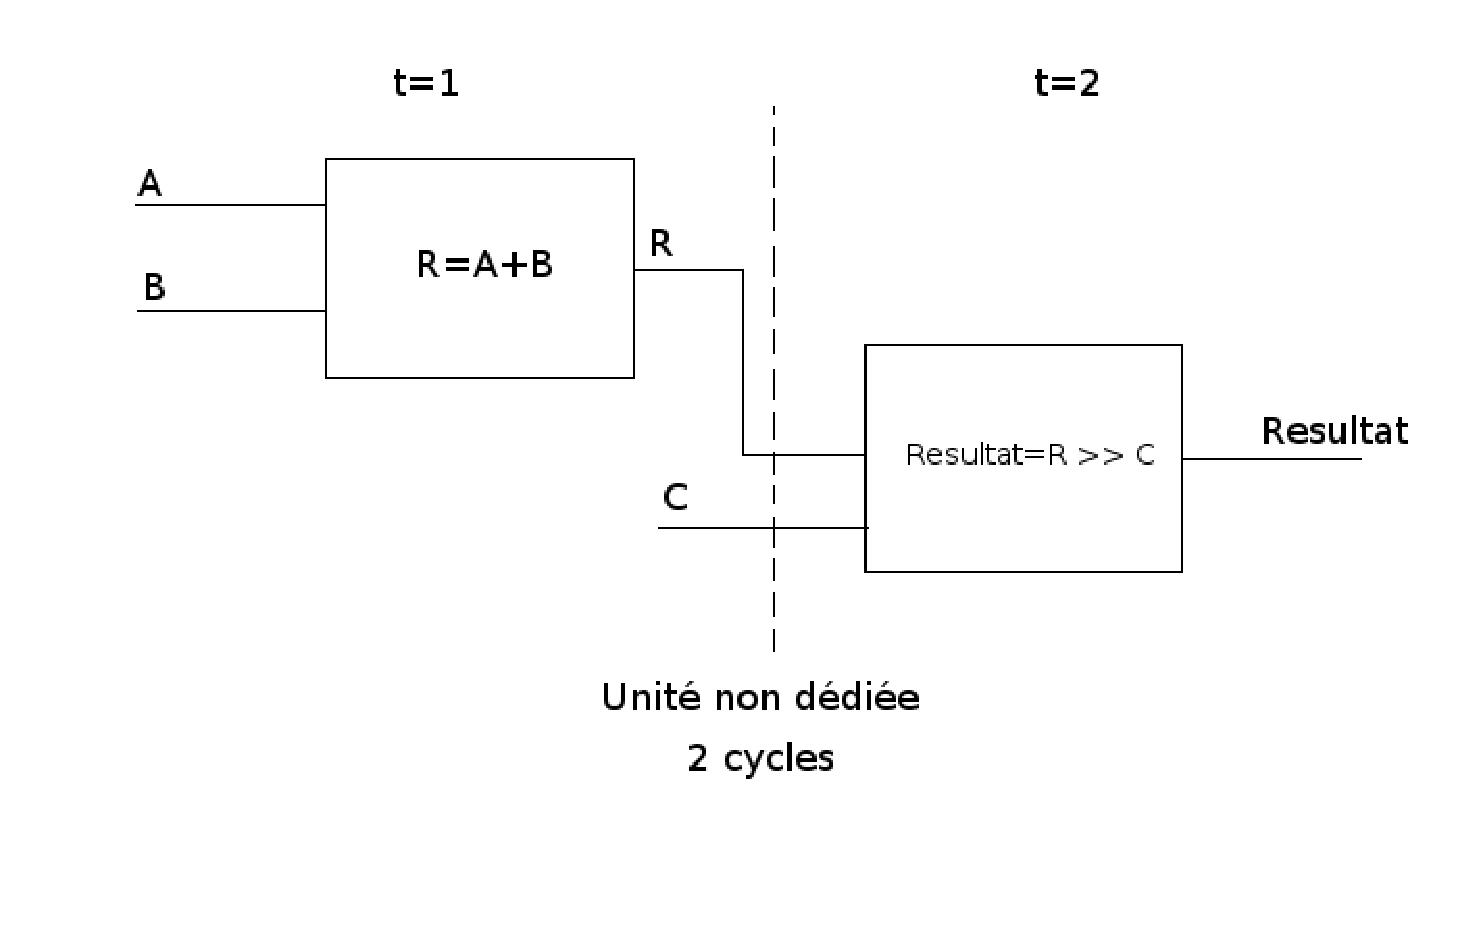
\includegraphics[scale=0.4]{bloc2.eps}

    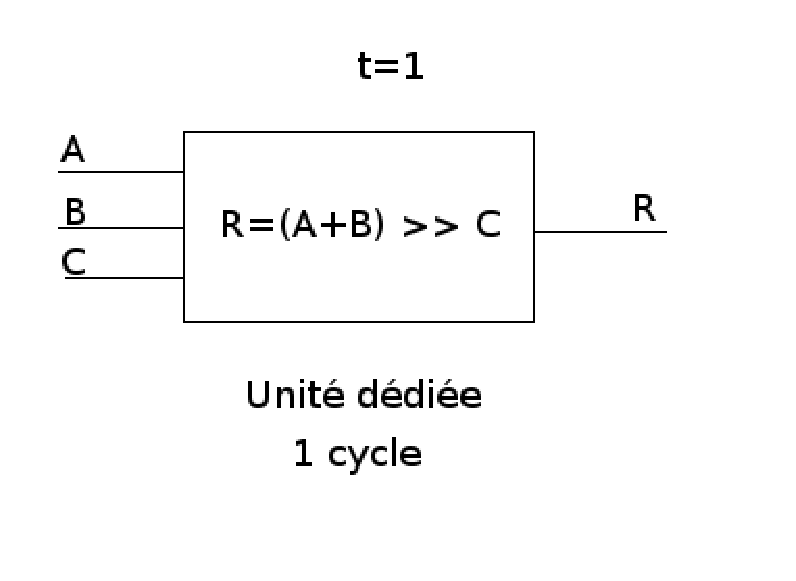
\includegraphics[scale=0.4]{bloc1.eps}

\end{center}
